\section{Einleitung}

In diesem Dokument wird das in der Veröffentlichung \enquote{The Serial Safety Net: Efficient Concurrency Control on Modern Hardware} von Wang et al. \cite{Wang:2015} vorgestellte Verfahren zur Sicherstellung der Serialisierbarkeit von Transaktionsplänen erläutert.
Dabei werden bestehende Concurrency-Control-Verfahren wie beispielsweise Snapshot-Isolation(SI), Read-Committed(RC) oder Read-Committed mit Locks(RCL) so erweitert, dass diese die Serialisierbarkeit der entstehenden Pläne gewährleisten.

Der Vorteil des Serial Safety Nets(SSN) gegenüber klassischen Verfahren, wie dem Zwei-Phasen-Sperrprotokoll(2PL) oder der Serializable-Snapshot-Isolation(SSI), besteht darin, dass eine bessere Nebenläufigkeit von Transaktionen ermöglicht wird, wodurch der Durchsatz des gesamten Systems massiv gesteigert wird.

\begin{figure}
	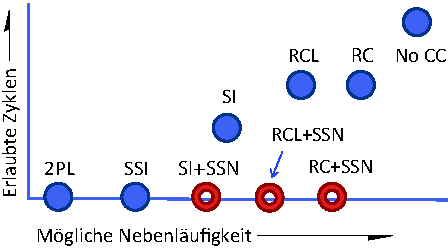
\includegraphics{img/Figure_1_komplett.pdf}
	\caption{Klassische Concurrency-Control-Verfahren im Vergleich zum Serial Safety Net}
	\label{fig:trade_off}
\end{figure}

In Abbildung \ref{fig:trade_off} wird schematisch dargestellt, dass ein bestimmter Trade-off zwischen der zugelassenen Nebenläufigkeit und den erlaubten Zyklen im Abhängigkeitsgraphen, also dem gewünschten Isolationslevel, besteht.
Klar erkennbar ist, dass ein optimales Concurrency-Control-Verfahren keinerlei Zyklen erlaubt und dennoch eine maximale Nebenläufigkeit gewährleistet.
Es wird deutlich, dass die durch das Serial Safety Net erweiterten Verfahren überhaupt keine solcher Zyklen erlauben und somit in dieser Hinsicht gleichwertig zu Verfahren wie 2PL und SSI sind.
Gleichzeitig ist allerdings erkennbar, dass die erlaubte Nebenläufigkeit wesentlich höher ist und somit ein Performanzgewinn erwartet wird.

Einige Gründe dafür, dass die bisher bekannten Verfahren zur Sicherstellung der Serialisierbarkeit, wenig performant sind, finden sich darin, dass diese einen hohen Overhead produzieren und teilweise zu unnötigen Transaktionsabbrüchen führen, wodurch möglicherweise gültige Pläne verworfen werden.
Außerdem funktionieren diese aufgrund schlechter Skalierung schlecht auf moderner Hardware, bei der immer mehr Operationen im Hauptspeicher stattfinden, wodurch die I/O-Last sinkt und damit ein noch größerer Fokus auf einem effizienten Concurrency-Control-System liegt.

Wichtig ist in diesem Zusammenhang zu erwähnen, dass ein Transaktionsplan, der in diesem Dokument als serialisierbar bezeichnet wird, keinen Schutz gegen Phantome bietet.
Das Serial Safety Net lässt sich durch das Verwenden von Sperren allerdings leicht erweitern, sodass das Vorkommen von Phantomen ausgeschlossen wird, worauf allerdings hier nicht weiter eingegangen werden soll.
Weitere Informationen zu möglichen Anomalien, Isolationsleveln und dem Phantom-Problem finden sich in \cite{Berenson:1995}.